% questions.tex —— 2011 年·全国新课标卷·理科 · 题目内容片段（无答案）
% 由 tools/generate_projects.py 依来源总账自 2011/2011_数学真题_全国新课标理_试题.md 生成，勿手改（改源 MD 后重跑）


\gkpart{数学}

\begin{gktip}
\textbf{来源说明}：本题面依据固定源 PDF 两页 A3 题面逐题转录，原卷印刷页码 685–686。固定源不附答案，答案和解析均由本库独立复算。

\textbf{图形说明}：第 3、6、18、22 题的原卷流程图、三视图或几何图重绘为 TikZ/PGFPlots 矢量图。图形标记所指的 PNG 不随仓库保存。
\end{gktip}

\gkpart{一、选择题}

\begin{question}
\gkti{1}复数 $\dfrac{2+i}{1-2i}$ 的共轭复数是\mbox{（　　）}

（A）$-\dfrac35i$\quad（B）$\dfrac35i$\quad（C）$-i$\quad（D）$i$

\end{question}
\begin{question}
\gkti{2}下列函数中，既是偶函数又在 $(0,+\infty)$ 单调递增的函数是\mbox{（　　）}

（A）$y=x^3$\quad（B）$y=|x|+1$\quad（C）$y=-x^2+1$\quad（D）$y=2^{-|x|}$

\Needspace{0.4\textheight}
\end{question}
\begin{question}
\gkti{3}执行如图的程序框图，如果输入的 $N$ 是 $6$，那么输出的 $p$ 是\mbox{（　　）}
\nopagebreak[4]
\begin{center}\begin{tikzpicture}[>=stealth,node distance=8mm and 13mm,scale=.78,
  every node/.style={font=\small}]
\node[draw,rounded corners,minimum width=18mm,minimum height=7mm] (start) {开始};
\node[draw,minimum width=25mm,minimum height=7mm,below=of start] (input) {输入 $N$};
\node[draw,minimum width=32mm,minimum height=7mm,below=of input] (init) {$k=1,\ p=1$};
\node[draw,minimum width=34mm,minimum height=7mm,below=of init] (mul) {$p=p\cdot k$};
\node[draw,diamond,aspect=2,below=of mul] (test) {$k<N$};
\node[draw,minimum width=25mm,minimum height=7mm,right=of test] (inc) {$k=k+1$};
\node[draw,minimum width=30mm,minimum height=7mm,below=of test] (out) {输出 $p$};
\node[draw,rounded corners,minimum width=18mm,minimum height=7mm,below=of out] (end) {结束};
\draw[->] (start)--(input)--(init)--(mul)--(test);
\draw[->] (test)--node[above] {是}(inc);
\draw[->] (inc) |- (mul);
\draw[->] (test)--node[right] {否}(out)--(end);
\end{tikzpicture}
\end{center}
\nopagebreak[4]
（A）$120$\quad（B）$720$\quad（C）$1440$\quad（D）$5040$

\end{question}
\begin{question}
\gkti{4}有 $3$ 个兴趣小组，甲、乙两位同学各自参加其中一个小组，每位同学参加各个小组的可能性相同，则这两位同学参加同一个兴趣小组的概率为\mbox{（　　）}

（A）$\dfrac13$\quad（B）$\dfrac12$\quad（C）$\dfrac23$\quad（D）$\dfrac34$

\end{question}
\begin{question}
\gkti{5}已知角 $\theta$ 的顶点与原点重合，始边与 $x$ 轴的正半轴重合，终边在直线 $y=2x$ 上，则 $\cos2\theta=$\mbox{（　　）}

（A）$-\dfrac45$\quad（B）$-\dfrac35$\quad（C）$\dfrac35$\quad（D）$\dfrac45$

\Needspace{0.4\textheight}
\end{question}
\begin{question}
\gkti{6}在一个几何体的三视图中，正视图和俯视图如下图所示，

则相应的侧视图可以为\mbox{（　　）}
\nopagebreak[4]
\begin{center}\begin{tikzpicture}[>=stealth,scale=.62]
\node[font=\scriptsize] at (-1.1,2.7) {正视图};
\draw[thick] (-2.2,0)--(-.2,0)--(-.2,2.2)--(-2.2,2.2)--cycle;
\draw[thick] (-1.2,0)--(-1.2,2.2);
\node[font=\scriptsize] at (-1.2,-.35) {俯视图};
\draw[thick] (-2.2,-1.1)--(-.2,-1.1)--(-.2,-.1)--(-2.2,-.1)--cycle;
\draw[dashed] (-1.2,-1.1)--(-1.2,-.1);
\foreach \x/\lab in {1.0/{(A)},4.0/{(B)},7.0/{(C)},10.0/{(D)}} {
  \node[font=\scriptsize] at (\x,2.55) {\lab};
  \draw[thick] (\x-.65,.25)--(\x,.25+1.65)--(\x+.65,.25)--cycle;
}
\draw[dashed] (3.35,.25)--(4.0,1.9)--(4.65,.25);
\draw[thick] (6.35,.25)--(7.0,1.9)--(7.65,.25);
\draw[dashed] (9.35,.25)--(10.0,1.9)--(10.65,.25);
\end{tikzpicture}
\end{center}
\nopagebreak[4]
（A）图 A\quad（B）图 B\quad（C）图 C\quad（D）图 D

\end{question}
\begin{question}
\gkti{7}设直线 $l$ 过双曲线 $C$ 的一个焦点，且与 $C$ 的一条对称轴垂直，$l$ 与 $C$ 交于 $A\text{、}B$ 两点，$|AB|$ 为 $C$ 的实轴长的 $2$ 倍，则 $C$ 的离心率为\mbox{（　　）}

（A）$\sqrt2$\quad（B）$\sqrt3$\quad（C）$2$\quad（D）$3$

\end{question}
\begin{question}
\gkti{8}$(x+\dfrac ax)(2x-\dfrac1x)^5$ 的展开式中各项系数的和为 $2$，则该展开式中常数项为\mbox{（　　）}

（A）$-40$\quad（B）$-20$\quad（C）$20$\quad（D）$40$

\end{question}
\begin{question}
\gkti{9}由曲线 $y=\sqrt{x}$、直线 $y=x-2$ 及 $y$ 轴所围成的图形的面积为\mbox{（　　）}

（A）$\dfrac{10}{3}$\quad（B）$4$\quad（C）$\dfrac{16}{3}$\quad（D）$6$

\end{question}
\begin{question}
\gkti{10}已知 $\boldsymbol a$ 与 $\boldsymbol b$ 均为单位向量，其夹角为 $\theta$，有下列四个命题：

\nopagebreak[4]
\[
\begin{aligned}
p_1 &: |\boldsymbol a+\boldsymbol b|>1\Longleftrightarrow \theta\in\left[0,\frac{2\pi}{3}\right),\qquad
p_2 &: |\boldsymbol a+\boldsymbol b|>1\Longleftrightarrow \theta\in\left(\frac{2\pi}{3},\pi\right],\\
p_3 &: |\boldsymbol a-\boldsymbol b|>1\Longleftrightarrow \theta\in\left[0,\frac\pi3\right),\qquad
p_4 &: |\boldsymbol a-\boldsymbol b|>1\Longleftrightarrow \theta\in\left(\frac\pi3,\pi\right].
\end{aligned}
\]

其中的真命题是\mbox{（　　）}

（A）$p_1,p_4$\quad（B）$p_1,p_3$\quad（C）$p_2,p_3$\quad（D）$p_2,p_4$

\end{question}
\begin{question}
\gkti{11}设函数 $f(x)=\sin(\omega x+\varphi)+\cos(\omega x+\varphi)$（$\omega>0$，$|\varphi|<\dfrac\pi2$）的最小正周期为 $\pi$，且 $f(-x)=f(x)$，则\mbox{（　　）}

（A）$f(x)$ 在 $\left(0,\dfrac\pi2\right)$ 单调递减

（B）$f(x)$ 在 $\left(\dfrac\pi4,\dfrac{3\pi}4\right)$ 单调递减

（C）$f(x)$ 在 $\left(0,\dfrac\pi2\right)$ 单调递增

（D）$f(x)$ 在 $\left(\dfrac\pi4,\dfrac{3\pi}4\right)$ 单调递增

\end{question}
\begin{question}
\gkti{12}函数 $y=\dfrac1{1-x}$ 的图象与函数 $y=2\sin\pi x$（$-2\leq x\leq4$）的图象所有交点的横坐标之和等于\mbox{（　　）}

（A）$2$\quad（B）$4$\quad（C）$6$\quad（D）$8$

\end{question}
\gkpart{二、填空题}

\begin{question}
\gkti{13}若变量 $x\text{、}y$ 满足约束条件

\nopagebreak[4]
\[
\begin{cases}
3\leq2x+y\leq9,\\
6\leq x-y\leq9,
\end{cases}
\]

则 $z=x+2y$ 的最小值为\gkblank{}。

\end{question}
\begin{question}
\gkti{14}在平面直角坐标系 $xOy$ 中，椭圆 $C$ 的中心为原点，焦点 $F_1\text{、}F_2$ 在 $x$ 轴上，离心率为 $\dfrac{\sqrt2}{2}$，过 $F_1$ 的直线 $l$ 交 $C$ 于 $A\text{、}B$ 两点，且 $\triangle ABF_2$ 的周长为 $16$，那么 $C$ 的方程为\gkblank{}。

\end{question}
\begin{question}
\gkti{15}已知矩形 $ABCD$ 的顶点都在半径为 $4$ 的球 $O$ 的球面上，且 $AB=6$，$BC=2\sqrt3$，则棱锥 $O-ABCD$ 的体积为\gkblank{}。

\end{question}
\begin{question}
\gkti{16}在 $\triangle ABC$ 中，$B=60^\circ$，$AC=\sqrt3$，则 $AB+2BC$ 的最大值为\gkblank{}。

\end{question}
\gkpart{三、解答题}

\begin{question}
\gkti{17}等比数列 $\{a_n\}$ 的各项均为正数，且 $2a_1+3a_2=1$，$a_2^3=9a_2a_6$。

（1） 求数列 $\{a_n\}$ 的通项公式；

（2） 设 $b_n=\log_3a_1+\log_3a_2+\cdots+\log_3a_n$，求数列 $\left\{\dfrac1{b_n}\right\}$ 的前 $n$ 项和。

\Needspace{0.4\textheight}
\end{question}
\begin{question}
\gkti{18}如图，四棱锥 $P-ABCD$ 中，底面 $ABCD$ 为平行四边形，$\angle DAB=60^\circ$，$AB=2AD$，$PD\perp$ 底面 $ABCD$。
\nopagebreak[4]
\begin{center}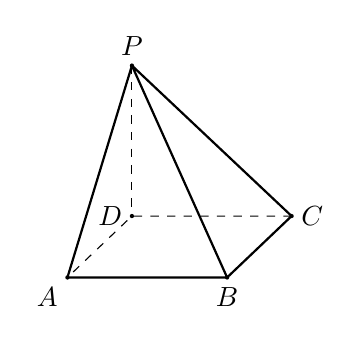
\begin{tikzpicture}[scale=.78,>=stealth]
\coordinate (A) at (0,0);
\coordinate (B) at (2.6,0);
\coordinate (C) at (3.65,1.0);
\coordinate (D) at (1.05,1.0);
\coordinate (P) at (1.05,3.45);
\draw[thick] (A)--(B)--(C);
\draw[dashed] (C)--(D)--(A);
\draw[thick] (P)--(A) (P)--(B) (P)--(C);
\draw[dashed] (P)--(D);
\fill (A) circle (1pt) node[below left] {$A$};
\fill (B) circle (1pt) node[below] {$B$};
\fill (C) circle (1pt) node[right] {$C$};
\fill (D) circle (1pt) node[left] {$D$};
\fill (P) circle (1pt) node[above] {$P$};
\end{tikzpicture}
\end{center}
\nopagebreak[4]
（1） 证明：$PA\perp BD$；

（2） 若 $PD=AD$，求二面角 $A-PB-C$ 的余弦值。

\end{question}
\begin{question}
\gkti{19}某种产品的质量以其质量指标值衡量，质量指标值越大表明质量越好，且质量指标值大于或等于 $102$ 的产品为优质品。现用两种新配方（分别称为 A 配方和 B 配方）做试验，各生产了 $100$ 件这种产品，并测量了每件产品的质量指标值，得到了下面试验结果：

\begin{center}
\begin{tabular}{lrrrrr}
\toprule
指标值分组 & $[90,94)$ & $[94,98)$ & $[98,102)$ & $[102,106)$ & $[106,110]$ \\
\midrule
A 配方的频数 & 8 & 20 & 42 & 22 & 8 \\
B 配方的频数 & 4 & 12 & 42 & 32 & 10 \\
\bottomrule
\end{tabular}
\end{center}

（1） 分别估计用 A 配方、B 配方生产的产品的优质品率；

\Needspace{5\baselineskip}
（2） 已知用 B 配方生产一件产品的利润 $y$（单位：元）与其质量指标值 $t$ 的关系式为

\nopagebreak[4]
\[
y=\begin{cases}
-2,&t<94,\\
2,&94\leq t<102,\\
4,&t\geq102.
\end{cases}
\]

从用 B 配方生产的产品中任取一件，其利润记为 $X$（单位：元），求 $X$ 的分布列及数学期望。（以实验结果中质量指标值落入各组的频率作为一件产品的质量指标值落入相应组的概率）

\end{question}
\begin{question}
\gkti{20}在平面直角坐标系 $xOy$ 中，已知点 $A(0,-1)$，$B$ 点在直线 $y=-3$ 上，$M$ 点满足 $\overrightarrow{MB}\parallel\overrightarrow{OA}$，$\overrightarrow{MA}\cdot\overrightarrow{AB}=\overrightarrow{MB}\cdot\overrightarrow{BA}$，$M$ 点的轨迹为曲线 $C$。

（1） 求 $C$ 的方程；

（2） $P$ 为 $C$ 上的动点，$l$ 为 $C$ 在 $P$ 点处的切线，求 $O$ 点到 $l$ 距离的最小值。

\end{question}
\begin{question}
\gkti{21}已知函数 $f(x)=\dfrac{a\ln x}{x+1}+\dfrac bx$，曲线 $y=f(x)$ 在点 $(1,f(1))$ 处的切线方程为 $x+2y-3=0$。

（1） 求 $a\text{、}b$ 的值；

（2） 如果当 $x>0$，且 $x\neq1$ 时，$f(x)>\dfrac{\ln x}{x-1}+\dfrac kx$，求 $k$ 的取值范围。

\Needspace{0.4\textheight}
\end{question}
\begin{question}
\gkti{22}如图，$D\text{、}E$ 分别为 $\triangle ABC$ 的边 $AB\text{、}AC$ 上的点，且不与 $\triangle ABC$ 的顶点重合。已知 $AE$ 的长为 $m$，$AC$ 的长为 $n$，$AD\text{、}AB$ 的长是关于 $x$ 的方程 $x^2-14x+mn=0$ 的两个根。
\nopagebreak[4]
\begin{center}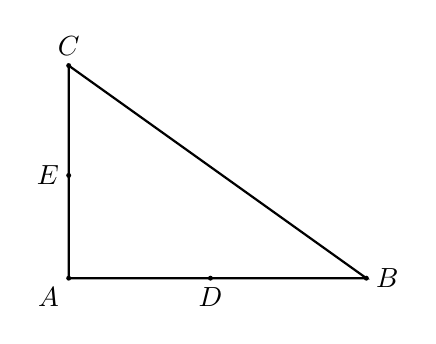
\begin{tikzpicture}[>=stealth,scale=.9]
\coordinate (A) at (0,0);
\coordinate (B) at (4.2,0);
\coordinate (C) at (0,3.0);
\coordinate (D) at (2.0,0);
\coordinate (E) at (0,1.45);
\draw[thick] (A)--(B)--(C)--cycle;
\fill (A) circle (1pt) node[below left] {$A$};
\fill (B) circle (1pt) node[right] {$B$};
\fill (C) circle (1pt) node[above] {$C$};
\fill (D) circle (1pt) node[below] {$D$};
\fill (E) circle (1pt) node[left] {$E$};
\end{tikzpicture}
\end{center}
\nopagebreak[4]
（1） 证明：$C\text{、}B\text{、}D\text{、}E$ 四点共圆；

（2） 若 $\angle A=90^\circ$，且 $m=4$，$n=6$，求 $C\text{、}B\text{、}D\text{、}E$ 所在圆的半径。

\end{question}
\begin{question}
\gkti{23}在直角坐标系 $xOy$ 中，曲线 $C_1$ 的参数方程为

\nopagebreak[4]
\[
x=2\cos\alpha,\qquad y=2+2\sin\alpha\quad(\alpha\text{ \text{为参数}}),
\]

$M$ 是 $C_1$ 上的动点，$P$ 点满足 $\overrightarrow{OP}=2\overrightarrow{OM}$，$P$ 点的轨迹为曲线 $C_2$。

（1） 求 $C_2$ 的方程；

（2） 在以 $O$ 为极点、$x$ 轴的正半轴为极轴的极坐标系中，射线 $\theta=\dfrac\pi3$ 与 $C_1$ 的异于极点的交点为 $A$，与 $C_2$ 的异于极点的交点为 $B$，求 $|AB|$。

\end{question}
\begin{question}
\gkti{24}设函数 $f(x)=|x-a|+3x$，其中 $a>0$。

（1） 当 $a=1$ 时，求不等式 $f(x)\geq3x+2$ 的解集；

（2） 若不等式 $f(x)\leq0$ 的解集为 $\{x\mid x\leq-1\}$，求 $a$ 的值。

\end{question}